\ylDisplay{Lääts} % Ülesande nimi
{Tundmatu autor} % Autor
{piirkonnavoor} % Voor
{2012} % Aasta
{P 10} % Ülesande nr.
{3} % Raskustase
{
% Teema: Valgusõpetus
\ifStatement
Klaasist kaksiknõgusa läätse optilisel peateljel paikneb väikeste mõõtmetega valgusallikas. Millist abivahendit, mis asub valgusallika ja nõgusläätse vahel, ja kuidas kasutades, saab nõgusläätse taha tekitada koonduva valgusvihu ja valgusallika tõelise kujutise? Põhjendage vastust joonisega.
\fi
\ifHint
Nõgusläätse ette tuleb paigutada koondav lääts, mille optiline peatelg ühtib nõgusläätse optilise peateljega.Koondava läätse optilise tugevuse arvuline väärtus peab olema suurem nõgusläätse optilise tugevuse arvulisest väärtusest, sest ainult sel juhul käitub kogu läätsede süsteem valgust koondavana.
\fi
\ifSolution
Nõgusläätse ette tuleb paigutada koondav lääts, mille optiline peatelg ühtib nõgusläätse optilise peateljega. Koondava läätse optilise tugevuse arvuline väärtus peab olema suurem nõgusläätse optilise tugevuse arvulisest väärtusest, sest ainult sel juhul käitub kogu läätsede süsteem valgust koondavana. Joonistame nõgusläätse optilise kõrvaltelje, mis on paralleelne nõgusläätsele langeva valguskiirega ja nõgusläätse eesmise fokaaltasandi. Nõgusläätsesele langev optilise kõrvalteljega paralleelne valguskiir murdub nõgusläätses nii, et selle kiire pikendus läbib punkti, kus lõikub nõgusläätse konkreetne optiline kõrvaltelg eesmise fokaaltasandiga. Analüüsime joonise abil kumerläätse ja nõgusläätse omavahelist asetust. Kuna hajutav ja koondav lääts asuvad teineteisest eemal, siis peab valgusallika kaugus koondavast läätsest olema selline, et koondavast läätsest langeks nõgusläätsele valguskiir, mis lõikuks läätsede optilise peateljega nõgusläätse ja selle tagumise fookuse vahel. Ainult sellisel juhul on valgusvihk ka pärast nõgusläätse koonduv.
\begin{center}
	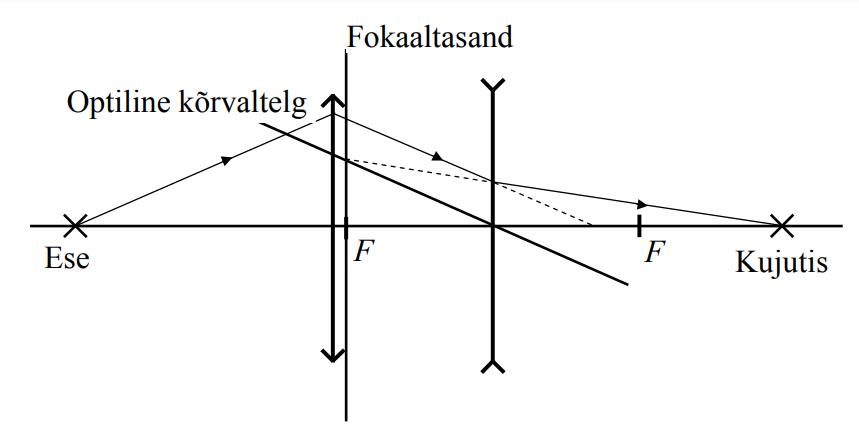
\includegraphics[width=0.5\linewidth]{2012-v2p-10-lah.PNG}
\end{center}
\fi
}
